\documentclass[a4paper,9pt,twocolumn]{ltjsarticle} % ← lualatex ではなく ltjsarticle
\usepackage[ipaex]{luatexja-preset}  % 日本語フォントの手当て(IPAex)
\usepackage{ifthen}
\usepackage{algorithm}
\usepackage{algorithmicx}
\usepackage{algpseudocode}
\usepackage{amsmath}
\usepackage{graphicx}
\usepackage{here}

\makeatletter
\renewcommand{\maketitle}{%
\ifthenelse{\equal{\course}{bachelor}}{%
  \begin{titlepage}
    \vspace*{10mm}
    \begin{center}
      {\huge\@gyear 年度\hspace{5mm}\@thesis\par}
      \vfill
      {\huge\bfseries\@title\par}
      \vfill
      \vspace{10mm}
      {\Large\@date\par}
      \vspace{20mm}
      {\Large\@department\@departmentsfx\par}
      {\Large (学生番号: \@studentid)\par}
      \vspace{5mm}
      {\LARGE\@author\par}
      \vspace{55mm}
      {\Large 和歌山大学\@faculty}
      \vspace{10mm}
    \end{center}
  \end{titlepage}}{}%
\ifthenelse{\equal{\course}{master}}{%
  \begin{titlepage}
    \begin{center}
      \vspace*{8mm}
      {\Large\@gyear 年度\hspace{5mm}\@thesis\par}
      \vfill
      {\huge\bfseries\@title\par}
      \vfill
      {\Large \@date\par}
      \vspace{40mm}
      {\Large 和歌山大学\@faculty\par}
      \vspace{27mm}
      {\Large 学生番号: \@studentid\par}
      {\LARGE \@author\par}
      \vspace*{28mm}
    \end{center}
  \end{titlepage}%
  \begin{titlepage}
    \begin{center}
      \vspace*{8mm}
      {\huge\@etitle\par}
      \vspace{12mm}
      {\Large by\par}
      \vspace{9mm}
      {\huge\@eauthor\par}
      \vspace{27mm}
      {\LARGE\@ethesis\par}
      \vfill
      {\Large \@efaculty\par}
      \vspace{4mm}
      {\Large Wakayama University\par}
      \vspace{23mm}
      {\Large \@edate\par}
      \vspace*{14mm}
    \end{center}
  \end{titlepage}}{}%
}

%% 概要
\def\abstract{\newpage\pagenumbering{roman}\section*{概 要}}
\def\endabstract{}
%% 目次
\def\tableofcontents{%
  \newpage
  \section*{目 次\@mkboth{目 次}{目 次}}
  \@starttoc{toc}}
%% 図目次
\def\listoffigures{%
  \newpage
  \section*{図 目 次\@mkboth{図 目 次}{図 目 次}}
  \@starttoc{lof}}
%% 表目次
\def\listoftables{%
  \newpage
  \section*{表 目 次\@mkboth{表 目 次}{表 目 次}}
  \@starttoc{lot}}
%% 謝辞
\def\acknowledgements{\newpage\section*{謝 辞}}
\def\endacknowledgements{}
%% 参考文献
\def\thebibliography#1{%
  \newpage
  \section*{参 考 文 献\@mkboth{参 考 文 献}{参 考 文 献}}
  \list{[\arabic{enumi}]}
    {\settowidth{\labelwidth}{[#1]}
     \leftmargin=\labelwidth
     \advance\leftmargin by \labelsep
     \usecounter{enumi}}
  \def\newblock{\hskip .11em plus .33em minus .07em}
  \sloppy
  \clubpenalty=4000 \widowpenalty=4000
  \sfcode`\.=1000\relax}
\let\endthebibliography=\endlist
\makeatother

\makeatletter
\def\course{bachelor}
\def\@gyear{2025}
\def\@thesis{卒業論文}
\def\@title{DIDに基づいたIoTデータ管理システムの構築と評価}
\def\@date{2026年2月10日}
\def\@department{システム工学部}
\def\@departmentsfx{システム工学科}
\def\@studentid{60276128}
\def\@author{竹内 結哉}
\def\@faculty{システム工学部}
\makeatother

\begin{document}
\maketitle

\section{はじめに}
近年,IoT機器の爆発的な増加に伴い,生成されるデータ量は急激に増加している.
さらに,IoTは家庭や産業,医療,農業など多様な分野で活用されるようになり,生成されるデータの種類や粒度も一層多様化している.

また,従来の中央集権型によるIoTデータ管理には,以下の3つの課題が存在する.
第一に,スケーラビリティの問題である.IoTデバイスの急増により,中央サーバーへの負荷が指数関数的に増大し,処理能力の限界に達する可能性がある.
第二に,セキュリティ上の問題である.中央サーバーは単一障害点となりやすく,攻撃対象として脆弱である.
第三に,プライバシー保護の問題である.個人情報を含むIoTデータが集中することで,情報漏洩時の被害が甚大化するリスクがある.

これらの課題を解決するために,本研究ではユーザー主権型IDに基づいた分散型データ管理システムの実現を目指す.
本システムは,以下の三点を重視して設計されている.

\begin{enumerate}
\item データの分散管理:中央集権型から脱却し,分散型ファイルシステムであるInterPlanetary File System(以下IPFS)を用いることで,
      単一障害点を排除しシステムの堅牢性を向上させる.
\item ユーザーの真正性確保:分散管理環境におけるなりすまし防止のため,分散型識別子であるDecentralized Identity(以下DID)を活用し,
      データ所有者の身元を保証する.
\item データの信頼性と改ざん防止:ブロックチェーンを活用し,データが改ざんされていないことを検証可能とする.
\end{enumerate}

以上の要素を組み合わせることで,IoTデータに対する分散型かつ信頼可能な管理基盤を構築することを目指す.

\section{関連研究}
IoTデータ管理におけるプライバシー確保は,従来より大きな研究課題とされている.
現行のIoTシステムは,多くが集中型のクライアントサーバーモデルに依存しており,生成される膨大なデータはサービスプロバイダを介して管理される.
このような集中型モデルは,ユーザーの行動履歴や個人情報が第三者に漏洩・不正利用されるリスクを内包している.
この問題に対処するため,近年ではブロックチェーンを基盤とした分散型データ管理アーキテクチャの研究が進められている.

Aliら\cite{cite1}は,ブロックチェーンとIPFSを組み合わせた\textbf{モジュラーコンソーシアムアーキテクチャ}を提案している.
このモデルでは,IoTデバイスをプライベートな「サイドチェーン」にグループ化し,アクセス制御の管理を「コンソーシアムブロックチェーン」によって実現する.
サイドチェーンはセンサーデータ生成イベントを記録し,コンソーシアムブロックチェーンはアクセス要求の不変なログを保持することで,
プライバシー保護とアカウンタビリティを両立させている.
さらに,データ自体はIPFS上に保存され,ブロックチェーンはハッシュのみを記録することで,ストレージ効率とセキュリティの両立を実現している.

評価実験として,Ethereum(PoW)およびMonax(PoS/Tendermint)を用いた性能比較が行われている.
その結果,Monaxはサイドチェーンレベルで低い処理オーバーヘッドを示す一方で,コンソーシアムレベルでは高いネットワークトラフィックオーバーヘッドが課題となった.
Ethereumはコンソーシアムレベルで通信効率に優れるものの,PoWに基づく高い計算コストが問題点として指摘されている.
このように,ブロックチェーンのコンセンサスメカニズムの選択は,IoT分散アーキテクチャの実用性に直接影響を与えることが明らかとなっている.

本研究は,この先行研究の知見を基盤としつつ,IoTデータ管理における\textbf{DID}と\textbf{VC}の統合に焦点を当てる.
既存研究が主に公開鍵基盤に依存したアクセス制御を行っていたのに対し,本研究ではDID/VCを導入することで,
より柔軟かつ標準化された認証・検証モデルを提供する点に新規性がある.
また,EthereumおよびIPFSを用いたローカル環境での実装と性能測定を通じて,スケーラビリティと実用性の両面から評価を行うことを目的としている.

\section{準備}
本研究では,分散型データ管理の基盤技術としてIPFS,DID,およびブロックチェーンを用いる.
本章では,これらの技術の概要を説明し,さらに本研究で使用した実験環境について述べる.

\subsection{IPFS}
IPFSは,分散型のファイルシステムであり,コンテンツ指向のアドレッシング方式を採用している.
従来のURLが「場所」に基づいてデータを参照するのに対し,IPFSではデータ内容から生成されるハッシュ値を用いて「内容」を参照する.
これにより,同一のデータは同一のハッシュ値で一意に識別され,データの改ざん検知が容易になるとともに,
ネットワーク上の複数ノードに分散保存することで耐障害性を高めることができる.
本研究では,IPFSの実装として\texttt{go-ipfs}を用いた.
これはIPFSの公式実装であり,Go言語で開発されている.

\subsection{DID}
DIDは,自己主権型アイデンティティを実現するための分散型識別子である.
従来のインターネットにおける認証・識別は,中央集権的な認証局やサービス提供者に依存していたため,
単一障害点や利用者のプライバシー保護に課題があった.
これに対しDIDは,ユーザー自身が管理可能な識別子を提供することで,第三者に依存せずに真正性を保証できる仕組みを実現する.
DID Documentと呼ばれる文書には公開鍵やサービスエンドポイントなどが含まれ,これにより利用者の認証やデータ検証を行うことができる.

\subsection{ブロックチェーン}
ブロックチェーンは,分散型台帳技術の一種であり,取引情報をブロックとして記録し,チェーン上に連結することで,
データの改ざん耐性を保証する.
各ブロックは暗号学的ハッシュにより前後のブロックと結合されており,一部のデータが改ざんされると以降のブロックすべてが不整合となるため,
改ざん検知が容易である.
また,ネットワークに参加する複数ノード間で合意形成を行い,信頼できる台帳を分散的に維持する仕組みを持つ.
本研究では実験環境としてEthereum互換のローカルブロックチェーン環境である\texttt{Ganache}を使用した.
Ganacheは開発用に特化したブロックチェーンシミュレータであり,高速なテスト実行やトランザクションの記録確認を容易に行うことができる.

\section{システム構成}
本研究で提案するシステムは,IoTデータを分散的に管理するために,DID,IPFS,およびブロックチェーンを連携させたものである.
本章では,まずシステム全体の流れを示した後,各要素の役割について説明する.

\subsection{全体像}
本研究で提案するシステムの全体像を図\ref{fig:system-overview}に示す.
\ref{fig:system-overview}に示すように,ユーザーAは自身のIoTデータをIPFSに格納し,その結果として得られるハッシュ値(以下CID)を,
自身の識別子であるDIDとともにブロックチェーンに記録する.
その後,発行者であるユーザーBがユーザーAの真正性を保証するVerifiable Credential(以下VC)を発行し,
検証者であるユーザーCがブロックチェーン上のDID情報とVCを突き合わせることで,ユーザーAの正当性を検証する.

\begin{figure}[H]
  \centering
  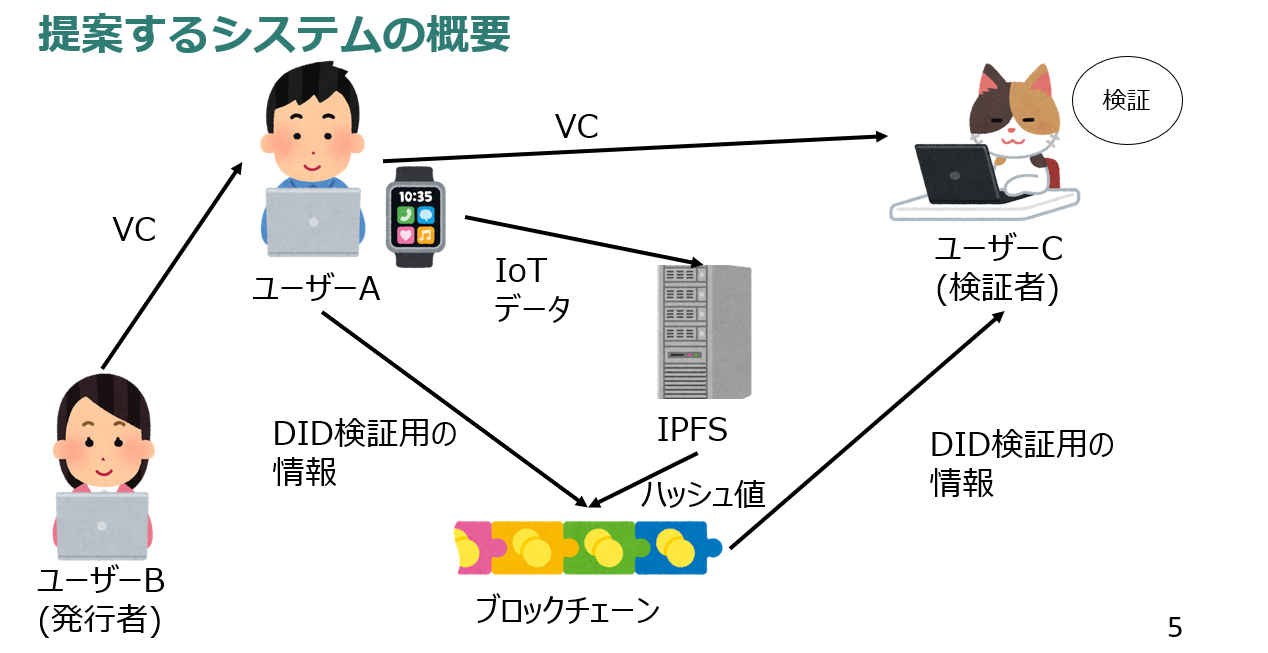
\includegraphics[width=0.9\linewidth]{figure1.png}
  \caption{提案システムの全体像}
  \label{fig:system-overview}
\end{figure}

\subsection{ユーザーA(データ所有者)}
ユーザーAは,自身の識別子としてDIDを保持し,その検証用情報(公開鍵など)をブロックチェーンに格納する.
さらに,所持しているIoTデータをIPFSに格納し,IPFSから返されるCIDを取得する.
このCIDはデータの一意なハッシュ値であり,データ改ざん検知に利用できる.
ユーザーAは,CIDと自身のDIDを組み合わせてブロックチェーンに登録することで,データの所有者であることを保証する.

\subsection{ユーザーB(発行者)}
ユーザーBは,発行者として,ユーザーAの真正性を保証する役割を担う.
ユーザーBは,ユーザーAのDIDに基づきVCを発行する.
このVCには,ユーザーAが正当な主体であることを示す署名が含まれており,第三者による検証を可能にする.

\subsection{ユーザーC(検証者)}
ユーザーCは,検証者として,ユーザーAから提示されたVCを受け取り,
ブロックチェーン上に記録されたDID検証用情報と突き合わせて検証を行う.
これにより,ユーザーAが正当なデータ所有者であることを確認できる.
この仕組みによって,IoTデータの分散的な流通においてもユーザーの信頼性とデータの真正性が担保される.

\subsection{データフロー}
本システムの具体的な処理の流れを図\ref{fig:system-flow}に示す.
\ref{fig:system-overview}に示すように,ユーザーAはIoTデータをIPFSに格納し,得られたCIDと自身のDIDをブロックチェーンに登録する.
その後,ユーザーBがVCを発行し,ユーザーAはこれをユーザーCに提示する.
ユーザーCはブロックチェーン上のDID情報とVCを照合することで,ユーザーAの正当性を検証する.

\begin{figure}[H]
  \centering
  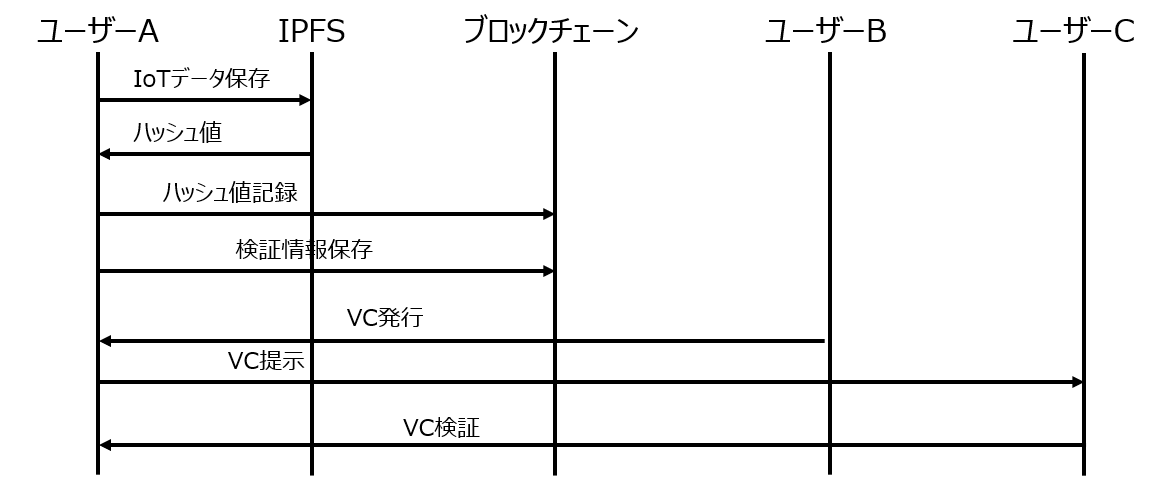
\includegraphics[width=0.95\linewidth]{figure2.png}
  \caption{データフロー図}
  \label{fig:system-flow}
\end{figure}

\section{実験と考察}

\subsection{実験目的}
本実験の目的は,提案システムにおける各処理の政党を定量的に評価し,
実社会での適用に耐えうる処理速度を有しているかを検証することである.
特に,IoTデータの分散保存にかかる処理時間,
DIDおよびVCを用いたユーザー検証の処理時間,
およびブロックチェーンにおけるトランザクション処理時間を測定対象とした.

\subsection{実験環境}
実験は以下の環境で行った.
\begin{itemize}
  \item OS:Windows 11 Home
  \item CPU:AMD Ryzen 5 PRO 7530U with Radeon Graphics(2.00Hz)
  \item メモリ:16GB
  \item IPFS:go-ipfs v0.35.0
  \item ブロックチェーン環境:Ganache v7.9.2
  \item Solidity: v0.5.16
  \item Node.js: v18.20.7
  \item Truffle: v5.11.5
  \item Web3.js: v1.10.0
\end{itemize}

\subsection{実験方法}
IPFS,DID,VC,ブロックチェーンに対応する各処理について,
ベンチマークスクリプトを用いて10回の測定を行い,平均時間を算出した.
測定対象は以下のとおりである.

\begin{enumerate}
  \item IoTデータ(約2.7KB)のIPFSアップロード処理
  \item ユーザーAに対するVC発酵処理
  \item ユーザーAのVC検証処理
  \item DID登録および発行に関するブロックチェーン処理
\end{enumerate}

\subsection{実験結果}
表\ref{tab:benchmark}に各処理の平均処理時間を示す.

\begin{table}[H]
  \centering
  \caption{各処理のベンチマーク結果(平均値)}
  \label{tab:benchmark}
  \resizebox{\linewidth}{!}{
  \begin{tabular}{l|r|l}
    \hline
    処理内容 & 平均処理時間 & 備考 \\
    \hline
    IPFSアップロード & 63.0ms & 2.7KBデータ,0.044 MB/s \\
    VC発行 & 5.99ms & 10回平均 \\
    VC検証 & 93.7ms & 10回平均 \\
    DID登録 & 88.2ms & gasUsed = 253{,}446 \\
    DID発行 & 46.6ms & gasUsed = 49{,}928 \\
    \hline
  \end{tabular}}
\end{table}

IPFSへのアップロードはデータサイズ2.7KBの場合に平均63.0msであり,
スループットは0.044 MB/sであった.
VC発行処理は平均5.99msと高速に実行可能であったのに対し,VC検証処理は平均93.7msを要した.
また,ブロックチェーンへのDID登録は平均88.2ms,DID発行処理は46.6msであり,
いずれも100ms未満で処理可能であった.

\subsection{考察}

\section{まとめ}

\bibliographystyle{junsrt}
\bibliography{references}
\end{document}
